\documentclass{article}

% if you need to pass options to natbib, use, e.g.:
%     \PassOptionsToPackage{numbers, compress}{natbib}
% before loading neurips_2023

\usepackage[preprint]{neurips_2023}


% to compile a preprint version, e.g., for submission to arXiv, add add the
% [preprint] option:
%     \usepackage[preprint]{neurips_2023}
% to compile a camera-ready version, add the [final] option, e.g.:
%     \usepackage[final]{neurips_2023}
% to avoid loading the natbib package, add option nonatbib:
%    \usepackage[nonatbib]{neurips_2023}
\usepackage[utf8]{inputenc} % allow utf-8 input
\usepackage[T1]{fontenc}    % use 8-bit T1 fonts
\usepackage{hyperref}       % hyperlinks
\usepackage{url}            % simple URL typesetting
\usepackage{booktabs}       % professional-quality tables
\usepackage{amsfonts}       % blackboard math symbols
\usepackage{nicefrac}       % compact symbols for 1/2, etc.
\usepackage{microtype}      % microtypography
\usepackage{xcolor}         % colors
\usepackage{svg}

\usepackage{algorithm}
\usepackage{algpseudocode}
\usepackage{amsmath}
\usepackage{todonotes}
\usepackage{enumitem}

\renewcommand\refname{Referencias}

\makeatletter
\renewcommand{\ALG@name}{Algoritmo}
\renewcommand{\figurename}{Figura}
\renewcommand{\tablename}{Tabla}
\makeatother

\title{Análisis de Redes}

% The \author macro works with any number of authors. There are two commands used to separate the names and addresses of multiple authors: \And and \AND.

\author{%
  Tomás Bossi\\
  \texttt{tomasbossi97@gmail.com} \\
  \And
  Francisco Valentini \\
  \texttt{ft.valentini@gmail.com} \\
  \And
  Jazmín Vidal \\
  \texttt{jazmin.vidald@gmail.com} \\
}

\begin{document}

\maketitle

\begin{abstract}
Este informe se centra en el análisis de redes mediante el cálculo de autovalores y autovectores. En primer lugar, presentamos los conceptos fundamentales sobre redes y la relevancia de los autovectores y autovalores en el análisis de estas estructuras. Luego, describimos el método de la potencia con deflación para hallar autovectores y autovalores, presentamos una implementación y estudiamos su desemepeño. Por último, exploramos diversas aplicaciones en el análisis de dos redes, el club de Karate \citep{zachary1977information} y Facebook \citep{leskovec2012learning}, incluyendo la medición de la centralidad de nodos, la evaluación de la conectividad y la comparación de redes a través de la correlación de autovalores. También abordamos la reducción de la dimensionalidad de matrices de atributos mediante el Análisis de Componentes Principales (PCA), técnica que se vale del cálculo de autovectores.
\end{abstract}

\section{Introducción} \label{sec:intro}

% [redes]
Podemos definir una red como el conjunto de los componentes de un sistema, típicamente llamados nodos o vértices, y de las interacciones entre ellos, denominadas aristas \citep{barabasi2013network}. Las redes pueden representar sistemas de distinta naturaleza, como redes sociales, redes de transporte, redes de comunicación, redes biológicas, etc. 

% [matriz de adyacencia]
El conjunto de aristas de una red se puede representar mediante una matriz de adyacencia. La matriz de adyacencia $A \in \mathbb{R}^{n \times n}$ de una red con $n$ vértices es una matriz cuyas entradas $A_{ij}$ son cero o uno, dependiendo de si los vértices $i$ y $j$ están conectados o no: $A_{ij} = 1$ si hay un arista desde el nodo $i$ hacia el nodo $j$, y $A_{ij} = 0$ si los nodos $i$ y $j$ no están conectados. 

En este informe nos circunscribimos a redes no dirigidas. Para este tipo de red, la matriz de adyacencia tiene dos entradas iguales para cada arista de la red porque el arista $(i, j)$ se representa como $A_{ij} = 1$ y $A_{ji} = 1$. Por lo tanto, la matriz de adyacencia de una red no dirigida es simétrica, $A=A^T$.

% [autovectores y autovalores]
La ecuación de autovalores de la matriz $A$ viene dada por $A v = \lambda v$, donde el número $\lambda \in \mathbb{R}$ es un autovalor y el vector $v \in \mathbb{R}^{n}$ es el autovector asociado. Si $A$ es simétrica, sabemos que tiene todos sus autovalores $\lambda_1, \ldots, \lambda_n$ reales y que sus autovectores asociados $v_1, \ldots, v_n$ forman una base ortonormal \citep{strang2022introduction}. Podemos ordenar los $\lambda_i$ de manera tal que $|\lambda_1| \geq |\lambda_2| \geq \ldots \geq |\lambda_n|$. Si se cumple que $|\lambda_1| > |\lambda_2|$, $\lambda_1$ es el autovalor dominante y $v_1$, el autovector dominante de $A$.

%\todo[inline]{por ser simetrica podemos asumir que hay un autovalor dominante? }
%Y que todos los autovalores son distintos?

% [método de la potencia]
Si $A$ tiene un autovalor dominante, entonces podemos encontrar a éste y al autovector dominante usando el método de la potencia \citep{watkins2004fundamentals}. La idea es elegir un vector inicial $q$ y formar la secuencia $q, Aq, A^2q, A^3q, \ldots$, de manera que cada vector en la secuencia se obtiene multiplicando el vector anterior por $A$, es decir: $A^{k+1}q = A(A^{k}q)$. 

Dado que $v_1, \ldots, v_n$ forman una base por tratarse de una matriz simétrica podemos encontrar constantes $c_1, \ldots, c_n$ tales que $q = c_1 v_1 + \ldots + c_n v_n$. Multiplicando por $A$, tenemos que:
%
$$
Aq = c_1 A v_1 + \ldots + c_n A v_n = c_1 \lambda_1 v_1 + \ldots + c_n \lambda_n v_n
$$
%
porque $A v_i = \lambda_i v_i$ para $i = 1, \ldots, n$. Si seguimos multiplicando por $A$, obtenemos
%
\begin{equation} \label{eq:potencia_ecuacion}
\begin{split}
  A^k q &= c_1 \lambda_1^k v_1 + c_2 \lambda_2^k v_2 + \ldots + c_n \lambda_n^k v_n \\
        &= \lambda_1^k (c_1 v_1 + c_2 ({\lambda_2}/{\lambda_1})^k v_n + \ldots + c_n ({\lambda_n}/{\lambda_1})^k v_n).
\end{split}
\end{equation}
%
Dado que los vectores son direcciones, podemos escalar por $\lambda_1^{-k}$, llegando así a
%
\begin{align*}
   A^k q / \lambda_1^{k} = c_1 v_1 + 
    c_2 ({\lambda_2}/{\lambda_1})^k v_n + 
    \ldots +
    c_n ({\lambda_n}/{\lambda_1})^k v_n.
\end{align*} 

Como $|\lambda_1| > |\lambda_i|$ para $i = 2, \ldots, n$, los términos $({\lambda_i}/{\lambda_1})^k$ tiende a cero cuando $k \to \infty$, y el componente en la dirección de $v_1$ domina en relación a los otros componentes. Es decir, para $k$ suficientemente alto, $A^k q / \lambda_1^{k}$ es una buena aproximación del autovector dominante. 

En la práctica, la secuencia $q_k = A^k q / \lambda_1^{k}$ es inaccesible porque no conocemos $\lambda_1$ de antemano. Además, $||A^k q|| \to \infty$ si $|\lambda_1| > 1$ y $||A^k q|| \to 0$ si $|\lambda_1| < 1$, por lo cual $q_k$ puede volverse demasiado grande o demasiado pequeño, generando underflow o overflow. Por lo tanto, en la práctica usamos algún tipo de normalización para obtener el autovector dominante, por ejemplo: 
%
\begin{equation} \label{eq:potencia_autovector}
    q_{k+1} = A q_{k} / ||A q_{k}||_{2}
\end{equation}
%
Y al usar la norma-2, la cantidad que converge al autovalor dominante $\lambda_1$ es:
%
\begin{equation} \label{eq:potencia_autovalor}
    \lambda_k = q_k^T A q_k / q_k^T q_k
\end{equation}

%\todo{Revisar, no estoy tan seguro.} A su vez, se puede demostrar que la secuencia converge hacia un autovector dominante para casi todas las elecciones iniciales de $q$ \citep{watkins2004fundamentals}. 

Resumiendo, dado un vector $q_0$ inicial, el método de la potencia nos devuelve un vector $q_k = A q_{k-1} / ||A q_{k-1}||_{2}$ que converge al autovector unitario $v_1$ de $A$, mientras que $\lambda_k = q_k^T A q_k / q_k^T q_k$ converge al autovalor dominante $\lambda_1$. 

% [deflacion]

Si además asumimos que $|\lambda_2| > |\lambda_3|$, podemos aplicar el método de deflación para obtener el segundo autovalor dominante $\lambda_2$ y su autovector asociado $v_2$. La idea es construir una matriz "desinflada" $A'$ a partir de $A$, $v_1$ y $\lambda_1$, y aplicar el método de la potencia a $A'$ para obtener $\lambda_2$ y $v_2$ \citep{watkins2004fundamentals}.

En particular, si consideramos $A' = A - \lambda_1 v_1 v_1^T$ vemos que $A'$ tiene autovalores $0, \lambda_2, \ldots, \lambda_n$ y autovectores asociados $v_1, v_2, \ldots, v_n$ porque 
%
$$
(A - \lambda_1 v_1 v_1^T) v_1 = A v_1 - \lambda_1 v_1 (v_1^T v_1) = \lambda_1 v_1 - \lambda_1 v_1 = 0 v_1
$$
y
$$
(A - \lambda_1 v_1 v_1^T) v_i = A v_i - \lambda_1 v_1 (v_1^T v_i) = \lambda_i v_i 
$$

El autovalor dominante de $A'$ es, entonces, $\lambda_2$ y su autovector asociado es $v_2$. Por lo tanto, podemos aplicar el método de la potencia descrito más arriba a $A'$ para obtener $\lambda_2$ y $v_2$. Aplicando este método iterativamente, obtenemos todos los autovalores y autovectores de $A$, siempre que se cumpla que $|\lambda_1| > |\lambda_2| > \ldots > |\lambda_n|$ y que los autovectores conformen una base ortonormal, lo cual es cierto si $A$ es simétrica.

% [centralidad de autovector]
Los autovalores y autovectores se pueden usar para caracterizar redes a partir de la matriz de adyacencia $A$. Por ejemplo, podemos usar el autovector dominante de $A$ para medir la centralidad de cada nodo de una red. Una medida de centralidad cuantifica la importancia de un vértice o nodo en una red. Intuitivamente, cuantos más vértices estén conectados a un nodo dado, mayor será su centralidad. Una propiedad adicional deseable es que la centralidad no dependa únicamente de las aristas directas hacia un nodo, sino que también dependa, de manera recursiva, de la centralidad de los nodos que apuntan hacia él \citep{zaki2014data}.

A partir de esta intuición de que la centralidad de un nodo depende de la centralidad de otros nodos que apuntan a él, podemos definir a $c_i$, la centralidad del vértice $i$, como:
%
\begin{equation} \label{eq:centralidad_i}
    c_i = \sum_{j=1}^{n} A_{ij} c_j
\end{equation}
%
donde $A \in \mathbb{R}^{n \times n}$ es la matriz de adyacencia simétrica. Nos restringimos a que $c_i$ sea un número real positivo \citep{zaki2014data}. Para todos los vértices en simultáneo, podemos expresar matricialmente y de manera recursiva la expresión \ref{eq:centralidad_i}:
%
\begin{align*}
    c' = A c
\end{align*}
%
donde $c$ es un vector de $n$ valores que indican la centralidad de cada vértice. Si comenzamos con un vector de centralidad inicial $c_{(0)}$, podemos usar esta ecuación para obtener un vector actualizado de manera iterativa: si $c_{(k-1)}$ es el vector de centralidad en la iteración $k - 1$, entonces el vector en la iteración $k$ se obtiene como:
%
\begin{equation} \label{eq:centralidad_secuencia}
\begin{split}
c_{(k)} &= A c_{(k-1)} \\
        &= A (A c_{(k-2)}) = A^2 c_{(k-2)} \\
        &= A^2 (A c_{(k-3)}) = A^3 c_{(k-3)} = \ldots \\
c_{(k)} &= A^k c_{(0)}
\end{split}
\end{equation}
%

Como hemos visto en la ecuación \ref{eq:potencia_ecuacion}, el vector $c_{(k)}$ converge al autovector dominante de $A$ a medida que aumenta $k$. El autovector dominante nos da, entonces, una medida de centralidad de los nodos de la red. Este autovector se puede obtener aplicando el método de la potencia.  
% [matriz laplaciana y vector de fiedler]

Otra manera de caracterizar una red es midiendo su conectividad. Para esto, podemos usar la matriz Laplaciana de la matriz de adyacencia $A$ que se define como $L = D - A$, donde $D$ es una matriz diagonal cuyos valores $d_{ii}$ indican la cantidad de aristas asociadas al vértice $i$. Se puede demostrar que para matrices de adyacencia simétricas, $L$ es simétrica y semidefinida positiva con todos autovalores iguales o mayores que cero, que la suma de sus filas y de sus columnas es cero y, considerando la ecuación de autovalores $L v = \lambda v$, podemos ver que el autovalor $\lambda = 0$ es un autovalor de $L$ y que su autovector asociado es un vector de unos \citep{dutta2022fiedler}. 

El autovalor más pequeño distinto de cero de $L$ se conoce como "conectividad algebraica" y su autovector asociado es el "vector de Fiedler", $v_F$. La magnitud de la conectividad algebraica refleja el grado de conectividad de la red. Por otra parte, el vector de Fiedler puede usarse para particionar una red en dos componentes densamente conectados. Esto se puede lograr separando los vértices $i$ en dos grupos: los que toman valores positivos $v_{Fi} > 0$ y los que toman valores negativos $v_{Fi} < 0$ \citep{dutta2022fiedler}.

% \todo{falta algo sobre Comparar redes mediante el cálculo de la correlación de autovalores?} --> NAa ya fue

Por último, introducimos la técnica de Análisis de Componentes Principales (PCA), la cual usamos para reducir la dimensión de una matriz de atributos. Dada una matriz de datos con $n$ observaciones y $p$ atributos, $X \in \mathbb{R}^{n \times p}$, PCA busca una base $r$-dimensional que maximice la varianza de los datos. La dirección con la mayor varianza proyectada se denomina primera componente principal. La dirección ortogonal que captura la segunda mayor varianza proyectada se denomina segunda componente principal, y así sucesivamente.

Para hallar estas direcciones podemos partir de la matriz de covarianza de $X$, la cual tiene la siguiente forma:
%
\begin{align*}
    \Sigma = \frac{1}{n-1} X_c^T X_c
\end{align*}
%
donde $X_c$ es la matriz de datos centrados, es decir, $X_c = X - \mu$, siendo $\mu$ es el vector de medias de los atributos. El valor $\Sigma_{ij}$ es la covarianza entre los atributos $i$ y $j$, y por lo tanto, el valor en la diagonal $\Sigma_{ii}$ es la varianza del atributo $i$. Es decir, $\Sigma$ es una matriz simétrica (y semidefinida positiva, ver \citealp{bishop2006pattern}). Al tratarse de una matriz con estas características, podemos diagonalizar la matriz de covarianza $\Sigma$ de los datos $X$ para obtener una base de autovectores $V$ y una matriz diagonal de autovalores $D$ tales que $\Sigma = V D V^T$. Asimismo, los autovectores forman una base ortonormal y los autovalores son todos no negativos y pueden ordenarse de manera decreciente tal que $\lambda_1 \geq \lambda_2 \geq \ldots \geq \lambda_p \geq 0$.

Las columnas de $V$ son los autovectores de $\Sigma$ y las componentes principales de los datos $X$. Para hallar una proyección de dimensión $k$ que maximice la varianza proyectada de los datos definimos una matriz $W = V_k \in \mathbb{R}^{p \times k}$, donde $V_k$ es la matriz que contiene los $k$ autovectores asociados a los $k$ autovalores más grandes de $\Sigma$. La proyección de los datos centrados $X_c$ en la matriz $W$ se obtiene como $Z = X_c W \in \mathbb{R}^{n \times k}$. Por medio de esta operación, obtenemos una matriz de datos $Z$ de dimensión reducida $k \leq p$ que captura la mayor varianza posible de los datos originales $X$.


\subsection{Objetivos del trabajo}

Los objetivos del presente trabajo son: 

\begin{enumerate}
    \item Implementar el método de la potencia con deflación para hallar autovectores y autovalores, analizando sus resultados y su convergencia en casos específicos de interés.
    \item Ilustrar el uso de los autovectores y autovalores para caracterizar redes en las siguientes aplicaciones: 
    \begin{enumerate}
        \item Medición de la centralidad de nodos. %de la red del Club de Karate.
        \item Medición de la conectividad de una red mediante el cálculo de los autovectores de la matriz Laplaciana. %de la red del club de Karate.
        % \item Particionar una red en dos componentes densamente conectados mediante el cálculo del vector de Fiedler de la matriz Laplaciana de la red del club de Karate.
        \item Comparación de redes midiendo la asociación entre su autovalores. %la red de amistades original y la construida a partir de los datos.  
        \item Reducción de la dimensionalidad de una matriz de atributos con PCA. %de los usuarios de Facebook.
    \end{enumerate}
\end{enumerate}

Para responder el segundo objetivo usamos los conjuntos de datos del Club de Karate \citep{zachary1977information} y de Facebook \citep{leskovec2012learning}

% , ambos correspondientes a dos matrices de adyacencia. 

%El método de la potencia está implementado en C++ y el análisis y la visualización de los datos en Python. 

La organización del trabajo se estructura de la siguiente manera: en la sección \ref{sec:desarrollo} describimos la implementación del método de la potencia con deflación y analizamos su desempeño (sección \ref{sec:algoritmos}), y presentamos los experimentos de aplicación de autovectores y autovalores en redes (sección \ref{sec:aplicaciones}). En la sección \ref{sec:resultados} presentamos los resultados de los experimentos. Finalmente, concluimos el trabajo en la sección \ref{sec:conclusiones}. 


\section{Desarrollo} \label{sec:desarrollo}

En la primera subsección presentamos el pseudocódigo del algoritmo del método de la potencia con deflación. Evaluamos la implementación en matrices donde los autovectores y autovalores son conocidos de antemano, y analizamos la convergencia en casos con autovalores repetidos y autovalores cercanos. En la segunda subsección presentamos los experimentos que ilustran la relevancia del cálculo de autovalores y autovectores para analizar redes tomando como caso el Club de Karate y la red de Facebook de un usuario. 


\subsection{Método de la potencia con deflación} \label{sec:algoritmos}

El pseudocódigo para el algoritmo que implementa el método de la potencia se define por las siguientes funciones:

\begin{algorithm}[!ht]
\caption{
    Método de la potencia para hallar el autovector dominante $v$ de $A$, dada una cantidad máxima de iteraciones ($niter$) y un valor para determinar la convergencia ($\epsilon$).
} 
\label{alg:potencia}
\begin{algorithmic}
\Function{MetodoPotencia}{$A$, $niter$, $\epsilon$}
    \State $numRows \gets \text{\# de filas de } A$
    \State $v \gets \text{Vector aleatorio de tamaño } numRows$ %\Comment{Autovector inicial}
    \For{$i \gets 0$ to $niter - 1$}
        \State $v\_previo \gets v$
        \State $v \gets A \cdot v$
        \State $v \gets \frac{v}{\|v\|}$ %\Comment{Normaliza el v}
        \If{$\left| v^T \cdot v\_previo - 1.0 \right| < \epsilon$}
            \State \textbf{break}
        \EndIf
    \EndFor
    \State \Return $v$
\EndFunction 
\end{algorithmic}
\end{algorithm}


\begin{algorithm}[!ht]
\caption{
    Función auxiliar para obtener el autovalor dominante $\lambda$ de $A$ asociado al autovector dominante $v$.
} 
\label{alg:potencia_autovalor}
\begin{algorithmic}
\Function{AutovalorDominante}{$A$, $v$}
    \State $scale \gets \|v\|^2$
    \State $\lambda \gets v^T \cdot A \cdot v$ 
    \State $\lambda \gets \frac{\lambda}{scale}$
    \State \Return $\lambda$
\EndFunction
 
\end{algorithmic}
\end{algorithm}

Inicialmente implementamos el método de la potencia para obtener el autovector dominante de una matriz cuadrada $A$ siguiendo la sucesión planteada en la ecuación \ref{eq:potencia_autovector} (algoritmo \ref{alg:potencia}). Para hallar el autovalor dominante dado el autovector dominante, usamos una función auxiliar que implementa la expresión \ref{eq:potencia_autovalor} (algoritmo \ref{alg:potencia_autovalor}). 


\begin{algorithm}[!ht]
\caption{
    Método de la potencia con deflación para hallar todos los autovalores y sus autovectores asociados.
} 
\label{alg:potencia_deflacion}
\begin{algorithmic}
\Function{PotenciaConDeflacion}{$A$, $num$, $niter$, $eps$}
    \State $numRows \gets \text{\# de filas de } A$
    \State $R \gets \text{Matriz de tamaño } (numRows + 1) \times numRows$ \Comment{Inicializa matriz de rdos.}
    \State $M \gets A$ \Comment{Inicializa matriz desinflada}
    \State $a \gets \text{Vector de tamaño } num$ \Comment{Vector de autovalores}
    \For{$i \gets 0$ to $num - 1$}
        \State $v \gets \text{MetodoPotencia}(M, niter, eps)$
        \State $\lambda \gets \text{AutovalorDominante}(M, v)$
        \State $R[i,:] \gets v^T$ \Comment{Asigna fila i-ésima}
        \State $a[i] \gets \lambda$ \Comment{Asigna elemento i-ésimo}
        \State $M \gets M - \lambda \cdot (v \cdot v^T)$ \Comment{Desinfla matriz}
    \EndFor
    \State $R[numRows,:] \gets a^T$ \Comment{Asigna última fila}
    \State \Return $R$
\EndFunction 
\end{algorithmic}
\end{algorithm}

Luego implementamos el método de potencia con deflación (algoritmo \ref{alg:potencia_deflacion}), el cual recibe como entradas una matriz $A$, los parámetros del método de la potencia, $niter$ y $\epsilon$, y la cantidad de autovalores a encontrar, $num$. La salida de esta función es una matriz $R \in \mathbb{R}^{(n+1) \times n}$ con los $n$ autovectores de $A$ en las primeras $n$ filas, y los autovalores asociados a cada uno, en la última fila, es decir:
%
\begin{equation*} \nonumber
    R =
    \begin{bmatrix}
                  &           & v_1^T  &               &           \\
                  &           & v_2^T  &               &           \\
                  &           & \vdots &               &           \\
                  &           & v_n^T  &               &           \\
        \lambda_1 & \lambda_2 & \cdots & \lambda_{n-1} & \lambda_n
    \end{bmatrix}
\end{equation*}
%

Estas funciones fueron implementadas en C++. Compilamos un programa con el compilador GCC 4.9 que recibe como argumento un archivo de texto con los datos de la matriz $A$, la cantidad de iteraciones ($niter$) y un valor de tolerancia para la convergencia ($\epsilon$). La salida son dos archivos de texto, uno con los autovalores y otro con los autovectores como columnas de una matriz. Para manipular matrices usamos la librería Eigen 3.4.0 \footnote{\url{https://eigen.tuxfamily.org/}}. 

Verificamos la implementación del método de la potencia en casos donde los autovalores y autovectores son conocidos. Para esto, armamos una matriz $M$ semejante a una matriz diagonal $D$ con los autovalores en la diagonal y los autovectores $Q$ y $Q^T$ multiplicando a izquierda y derecha tal que: 
$$
M = Q^T \begin{pmatrix}
\lambda_1    &0     &0      &0      \\
0      & \lambda_2   &0      &0      \\
\vdots &\vdots&\ddots &\vdots \\
0      &0     &0      & \lambda_n    \\
\end{pmatrix} Q
$$
con $Q = I - 2 v v^T$ y $||v||_2=1$, siendo $Q$ la matriz de reflexión (ortogonal) que hace las veces de matriz de autovectores. Además, comparamos estos autovectores y autovalores conocidos con los calculados usando el método  $linalg.eig$ de la biblioteca NumPy de Python, especializada en cálculo numérico eficiente.

En una primera exploración verificamos que se cumpla que $M v_i$ se aproxime a $M l_i$ para $i=1,\dots,n$, donde $l_i$ y $v_i$ son los autovalores y autovectores calculados con el algoritmo \ref{alg:potencia_deflacion}, respectivamente. En distintas matrices $M$ predeterminadas observamos que el método converge bien. Respecto de NumPy, observamos que nuestro método devuelve los mismos autovalores y autovectores, pero en algunas ocasiones no coincide en signo, es decir, devuelve otros sentidos de la misma dirección. 

%y en todos los casos realizamos una comparación entre $MV$ y $lV$ siendo $M$ la matriz que creamos y $l$ y $V$ los autovalores y autovectores que calculamos con cierta tolerancia.  

Más allá de esta primera verificación, analizamos la convergencia de nuestro método para casos de matrices con todos autovalores distintos. En particular, buscamos analizar el error en el cálculo de autovalores para distintos números de iteración y en comparación con NumPy. 

Planteamos un experimento que consiste en fijar el valor de convergencia en $\epsilon=0$ para aislar el impacto del número de iteraciones en el cálculo de los autovalores y autovectores. Luego, para los valores $niter=\{1, 10, 100, 1000, 2000, 5000, 10000\}$ calculamos los autovalores y autovectores de una matriz $M \in \mathbb{R}^{100 \times 100}$. Para cada uno de los 100 autovalores estimados para cada $niter$ y para NumPy, calculamos el valor absoluto del error relativo entre el autovalor real ($l_{true}$) y el calculado ($l_{est}$): $|(l_{est}-l_{true})/l_{true}|$.
% %
% \begin{equation} \nonumber
%     |(l_{est}-l_{true})/l_{true}|
%     \label{rel}
% \end{equation}
% %

Observamos que en nuestro método disminuye el error a medida que aumenta la cantidad de iteraciones, y que esto encuentra un límite en el orden de las $10^3$ iteraciones (Figura \ref{fig:convergencia_iguales}). NumPy tiene consistentemente menor error respecto de nuestos mejores casos.

Se analizó el caso particular de matrices con pares de autovalores muy parecidos entre sí, así como también el caso de matrices con autovalores repetidos. Para ello, se generaron al azar 100 matrices de tamaño $10 \times 10$ de autovalores y autovectores conocidos, y a partir de cada una se generaron matrices para las que se alteró sólo a $\lambda_2$, el segundo autovalor en orden de dominancia. Para matrices con autovalores parecidos se eligió $\lambda_2 = \lambda_1 - 10^{-10}$, y para matrices con autovalores repetidos se tomó $\lambda_2 = \lambda_1$. Para cada matriz se midió el error de la estimación de autovalores y autovectores como $\frac{\sum_{i=1}^{10}(Av_1 - \lambda_1v_1)_i^2}{10}$, es decir, como el error cuadratico medio (ECM) entre $Av_1$ y $\lambda_1v_1$.

En ambos casos se esperaba encontrar que la convergencia del método sea más lenta para estos tipos de matrices, es decir, que para una misma cantidad de iteraciones del método el error en la estimación sea mayor respecto a matrices con autovalores similares pero sin autovalores parecidos ni repetidos. Obtuvimos resultados contrarios a los esperados (figura \ref{fig:convergencia_patologica}), y al momento de escribir este informe no tenemos claro por qué.

% con una diferencia de $ $ 

\begin{figure}[!ht]
    \centering
        \includesvg[width=0.7\textwidth]{img/convergencia_autovalores.svg}
    \caption{
    Error relativo de estimación de autovalores en función de la cantidad de iteraciones del algoritmo \ref{alg:potencia_deflacion}, y de NumPy. Para cada condición se grafica, en forma de boxplot, la distribución de errores relativos (en módulo) entre los autovalores reales y los estimados.
    %El gráfico está en escala logaritmica. 
    } 
    \label{fig:convergencia_iguales}
\end{figure}

\begin{figure}[!ht]
    \centering
        \includesvg[width=0.49\textwidth]{img/convergencia_parecidos.svg}
        \includesvg[width=0.49\textwidth]{img/convergencia_repetidos.svg}
    \caption{
        Convergencia de la estimación del primer autovalor y autovector, medida como el error cuadrático medio entre $Av_1$ y $\lambda_1v_1$ en función de la cantidad de iteraciones del método. Cada punto representa el error promedio en la estimación para 100 matrices distintas, todas de tamaño $10 \times 10$. En azul: metrices con autovalores elegidos al azar. En naranja: matrices modificadas para que sus dos autovalores más dominantes sean muy parecidos entre sí (izquierda) o iguales (derecha), sin modificar al resto de los autovalores.
    } 
    \label{fig:convergencia_patologica}
\end{figure}

% \todo{REVISAR ESTE CAPTION:}

% \begin{figure}[ht!]
%     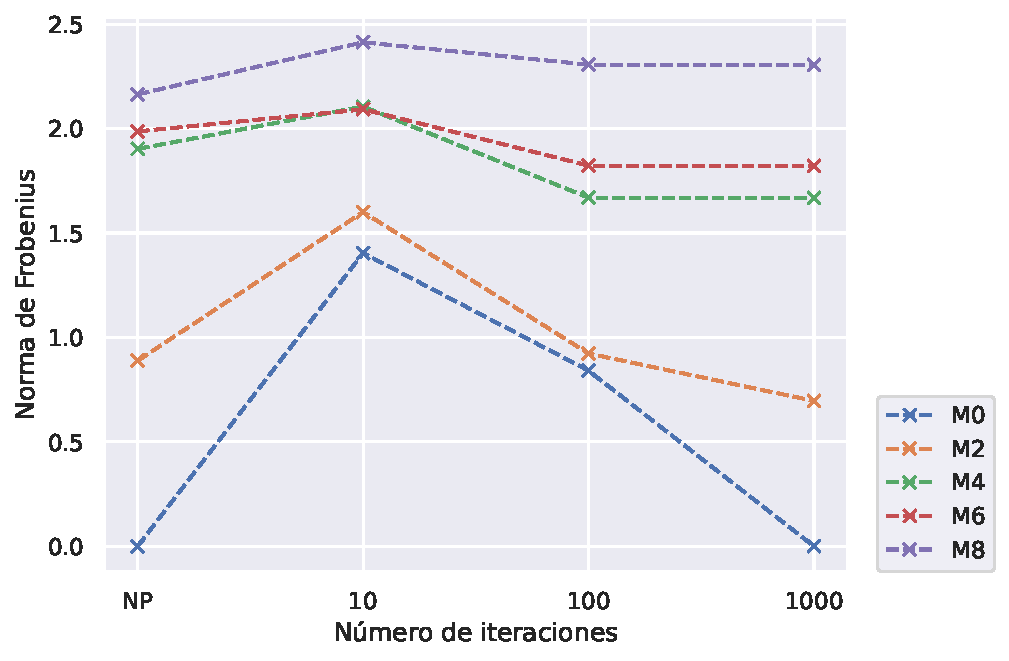
\includegraphics[width=0.33\linewidth]{img/frobenius.pdf}
%     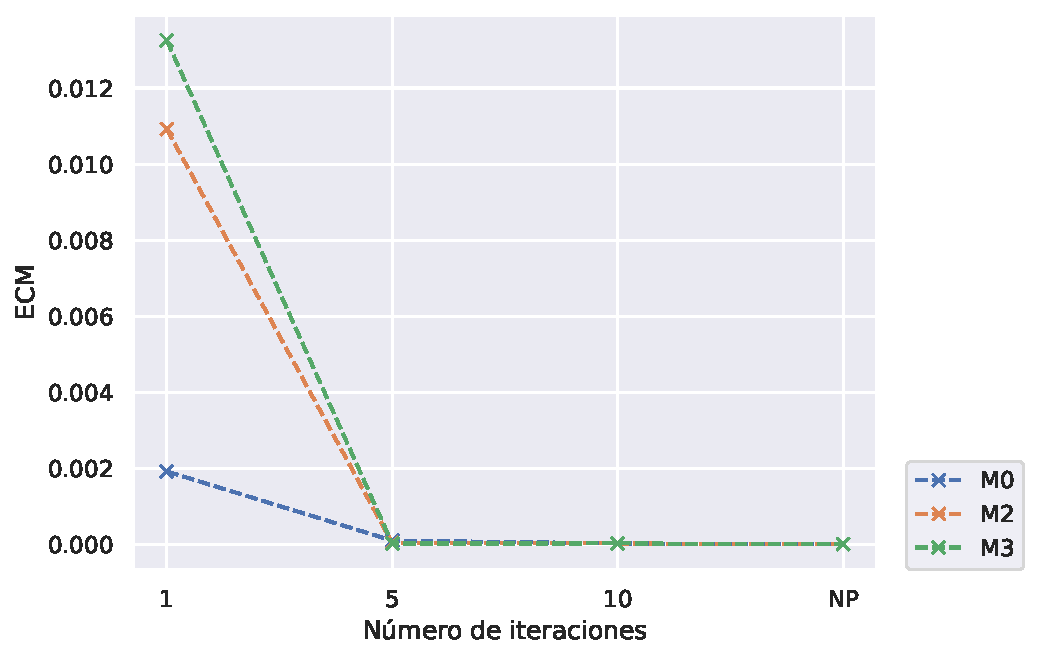
\includegraphics[width=0.33\linewidth]{img/mvlvconsec.pdf}
%     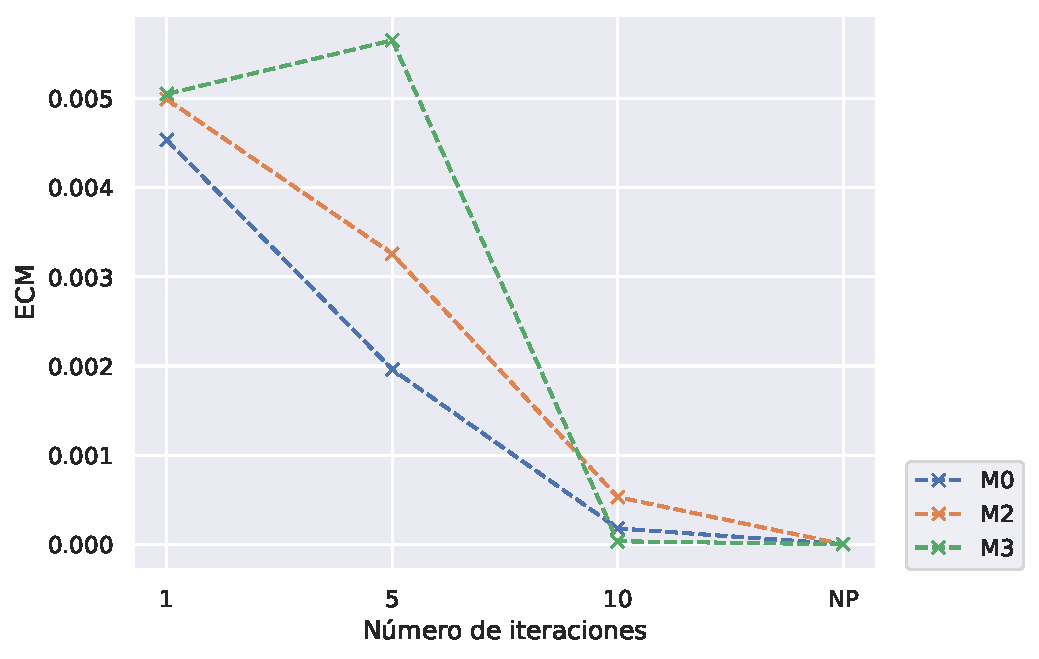
\includegraphics[width=0.33\linewidth]{img/mvlv2.pdf}
%     \caption{
%         Diferencia entre las matrices de autovectores correctas ($V_{GT}$) y las calculadas con el algoritmo \ref{alg:potencia_deflacion} y con NumPy ($V$), calculada como $\|V_{GT} - V\|_F$. A la izquierda, el autovalor dominante está repetido. En el medio, $ECM(AV_{gt}-l_{est}V_{gt}$. A la derecha,  $ECM(AV_{est}-l_{est}V_{est}$. El eje horizontal representa el método de cómputo (NP=NumPy, y algoritmo \ref{alg:potencia_deflacion} con distinta cantidad de iteraciones). Estudiamos los casos de 0, 2, 4, 6 y 8 autovalores repetidos.
%     }
%     \label{fig:repetidos_frobenius}
% \end{figure}

% \begin{figure}[!ht]
%     \centering
%     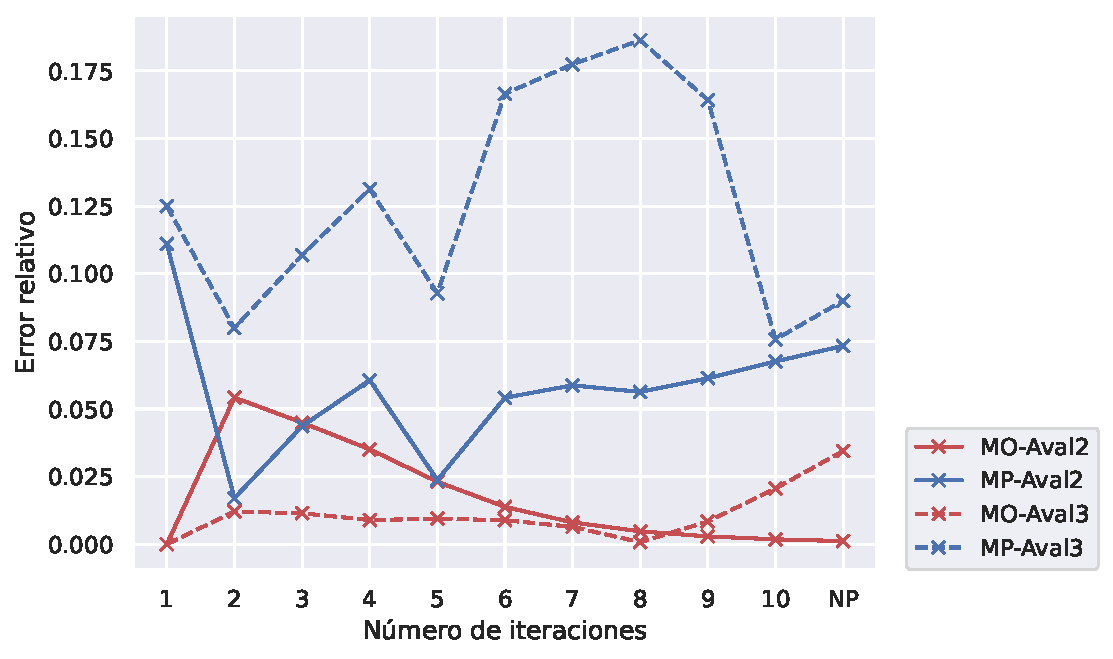
\includegraphics[width=0.7\textwidth]{img/error_rel.pdf}
%     \caption{
%     En el eje vertical, el error relativo del segundo autovalor y del tercer autovalor. En rojo, los resultados correspondientes a la matriz $M_O$ (sin autovalor cercano) y en azul los que corresponden a $M_P$ (con segundo y tercer autovalor parecidos). La línea indica el error del autovalor 2 y la punteada, del autovalor 3. En el eje horizontal, el número de iteraciones de 1 a 10 y los resultados correspondientes a NumPy (NP). 
%     } 
%     \label{fig:repetidos_relativo}
% \end{figure}

% \todo{REVISAR DESDE ACA}

% También experimentamos en casos de matrices con autovalores repetidos. Analizamos el caso en el que el primer autovalor dominante está repetido. Planteamos un experimento que consiste en diseñar 10 matrices $M_i \in \mathbb{R}^{5 \times 5}$ a las que le aumentamos progresivamente la cantidad de autovalores repetidos. Es decir, la matriz $M_0$ tiene todos autovalores distintos, la matriz $M_1$ tiene el autovalor dominante repetido dos veces, y así hasta llegar a un máximo de $M_8$. Construimos las matrices utilizando el método de ortogonalización descrito arriba para conocer los autovalores y autovectores de antemano. Llamamos a estas matrices de autovectores $V_{GT}$ donde $GT$ se refiere a "ground truth".

% Realizamos tres mediciones de error. En la primera (gráfico de la izquierda de la Figura \ref{fig:repetidos_relativo}), analizamos el error de NumPy y del algoritmo \ref{alg:potencia_deflacion} con $niter=\{10, 100, 1000\}$ y $\epsilon=0$ para aislar el comportamiento de la convergencia. En este caso nos interesa analizar el comportamiento de todos los autovectores predichos. Para eso tomamos como medida de error la norma de Frobenius de la matriz de diferencias entre la matriz de autovectores conocida $V_{GT}$ y la calculada $V$: 
% %
% \begin{equation} \nonumber
%     \|V_{GT} - V\|_F
% \end{equation}

% Luego, analizamos el error cuadrático medio de la diferencia entre $Av-lv$. En primer lugar, computamos esto usando $V_{GT}$ (panel central de la Figura \ref{fig:repetidos_relativo}). Esto permite aislar el efecto de la estimación de los autovalores. En segundo lugar, usamos V y l en el cálculo. 

% %Esto permite analizar de forma más general. 

% La Figura \ref{fig:repetidos_frobenius} muestra los resultados del experimento en los casos en el que el autovalor dominante está repetido (izquierda) y en el que algún otro autovalor está repetido (derecha). En ambos casos los resultados son similares. Por empezar, tanto NumPy como el método que implementamos muestran ser sensibles a la repetición de autovalores con una tendencia similar en la que el error aumenta a medida que lo hace el número de repeticiones. Por otro lado, se ve siempre un error más alto cuando el número de iteraciones es menor. 

% \todo{REVISAR HASTA ACA}

% Finalmente, analizamos la convergencia en casos con autovalores muy cercanos. Para esto, tomamos una matriz $M_O \in \mathbb{R}^{5 \times 5}$ y construimos una nueva matriz $M_P$ en la que el tercer autovalor es muy parecido al segundo. Por ejemplo, si la matriz $M_O$ tiene como vector de autovalores $l_O=[10,  9,  8,  7,  5]$, la matriz $M_P$ puede tener $l_P=[10,  9,  8.999,  7,  5]$, donde el tercer autovalor en la lista es muy cercano al segundo. Calculamos el error relativo entre cada autovalor real y el computado por NumPy y por nuestro método, y analizamos el error de los autovalores segundo y tercero para distinta cantidad de iteraciones (Figura \ref{fig:repetidos_relativo}). 

% Los errores en la matriz sin autovalores parecidos son más bajos en todos los casos y tienden a mejorar a medida que aumenta el número de iteraciones (curvas rojas). En cambio, cuando el segundo autovalor es similar al tercero (curvas azules), el error de cómputo promedio es sensiblemente más alto en el tercer autovalor que en el segundo, tanto al usar nuestro método como el método de NumPy. 

%%% Hasta acá estaba comentado lo viejo del 1.2 en su versión "final"

%Observamos los errores relativos para los dos autovalores consecutivos para las matrices $M_O$ y $M_P$. Vemos el error relativo para el segundo autovalor y su valor consecutivo en las dos matrices. En la primera se trata de un valor distinto, en la segunda de uno muy parecido. 


\subsection{Aplicaciones en redes} \label{sec:aplicaciones}

Nos proponemos ilustrar el uso del cálculo de autovalores y autovectores para caracterizar redes a partir de un conjunto de experimentos en dos conjuntos de datos: el "club de Karate"  y "Facebook".

\subsubsection{Club de Karate} \label{sec:karate}

El "Club de Karate" es una red social documentada por \citet{zachary1977information}, que resume los vínculos entre 34 miembros de un club de karate, en el cual se documentaron 78 aristas no dirigidas según las interacciones regulares entre los miembros fuera del club. Estas interacciones se pueden representar con una matriz de adyacencia $A \in \mathbb{R}^{78 \times 78}$, como explicamos en la sección \ref{sec:intro}. 

Durante el estudio ocurrió un conflicto que dividió al club en dos: la mitad de los miembros formaron un nuevo club mientras los miembros de la otra parte encontraron un nuevo instructor o abandonaron el karate. Por lo tanto, cada nodo está etiquetado según la pertencencia a cada uno de estos dos grupos post-conflicto.

%El interés del conjunto de datos se debe a un acontecimiento singular: Un conflicto entre el presidente del club y el instructor dividió al club en dos. Aproximadamente la mitad de los socios seguían al instructor y la otra mitad al presidente, una ruptura que desveló la verdad básica, que representa la estructura comunitaria subyacente del club (Imagen 9.2a).

Sobre este dataset hacemos los siguientes experimentos:

\begin{enumerate}[leftmargin=.5cm]
    
    \item Identificamos los nodos más centrales computando la centralidad de autovector con el algoritmo \ref{alg:potencia_deflacion}. Para esto, computamos el autovector dominante de la matriz de adyacencia $A$ como se describe en la sección \ref{sec:intro} (ecuación \ref{eq:centralidad_secuencia}).
    
    \item Buscamos el autovector de la matriz Laplaciana que mejor predice la pertenencia a los grupos post-conflicto. Para esto, medimos el valor absoluto de la correlación de Pearson entre cada autovector y el vector binario que indica la pertenencia a los grupos post-conflicto. Para encontrar los autovectores de la matriz Laplaciana usamos el algoritmo \ref{alg:potencia_deflacion} y comparamos con los resultados que se obtienen con la librería NumPy para Python \footnote{\url{https://NumPy.org/}}. 
    
\end{enumerate}


\subsubsection{Facebook} \label{sec:facebook}

El set de datos de usuarios de Facebook de \citet{leskovec2012learning} contiene una matriz de atributos $X \in \mathbb{R}^{n \times p}$ conformada por $n=792$ usuarios (filas) descritos por $p=319$ atributos binarios (columnas) que indican si el usuario tiene o no ciertas características. Para estos usuarios se cuenta también con una red no dirigida de amistades que se puede representar mediante una matriz de adyacencia simétrica $A \in \mathbb{R}^{792 \times 792}$, donde $A_{ij} = 1$ si el usuario $i$ es amigo del usuario $j$, y $A_{ij} = 0$ en caso contrario. 

A partir de la matriz de atributos computamos un matriz de similitud $S \in \mathbb{R}^{792 \times 792}$ donde $S_{ij}$ representa la similitud entre los usuarios $i$ y $j$ definida como el número de atributos en los que ambos usuarios tienen valor 1. Es decir, $S_{ij}$ se puede computar como el producto interno entre las filas $i$ y $j$ de la matriz de atributos $X$. Por lo tanto, $S$ se puede obtener como $S = XX^T$. 

Si fijamos un umbral de similitud $u$, podemos construir un grafo no dirigido donde los nodos son los usuarios y las aristas son las conexiones entre usuarios que tienen una similitud mayor o igual a $u$. Para este grafo obtenemos la matriz de adyacencia $A_S$. Por otra parte, es posible reducir la dimensionalidad de $X$ a $k$ dimensiones mediante PCA (ver sección \ref{sec:intro}) antes de obtener $S$ y $A_S$. Llamamos a la matriz de adyacencia que obtenemos mediante este método $A_S^k$.  

% Trabajamos inicialmente con un umbral fijado a priori de $t = XYZ$. \todo{completar}

Llevamos a cabo los siguientes experimentos:

\begin{enumerate}[leftmargin=.5cm]

    \item Buscamos el valor del umbral $u$ que optimiza la similitud entre la red de amistades (representada por $A$) y la red construida a partir de los atributos (representada por $A_S$). 

    Medimos la similitud entre redes para cada umbral usando dos métricas: (1) la correlación de Pearson de las matrices de adyacencia "estiradas" en un vector, y (2) la correlación de Pearson entre los vectores de autovalores ordenados de mayor a menor. Para obtener los autovalores usamos el algoritmo \ref{alg:potencia_deflacion} y validamos los resultados con la librería NumPy. 
    
    \item Analizamos cómo la proyección de $X$ a sus $k$ primeras componentes principales afecta a la búsqueda del umbral $u$ que optimiza las métricas de correlación. En particular, para distintas cantidades de componentes principales $k$ examinamos cómo varía la correlación en función de $u$.   

\end{enumerate}

Realizamos todos los análisis y visualizaciones usando Python. Para graficar las redes usamos la biblioteca networkx \footnote{\url{https://networkx.org/}}.

% \todo[inline]{ponemos hipotesis?}


\section{Resultados} \label{sec:resultados}

En esta sección presentamos los resultados de los análisis propuestos en la sección \ref{sec:aplicaciones}. 

% \todo[inline]{
%     Usamos gráficos y analizamos si se cumplieron o no las hipótesis que formulamos?
% }


\subsection{Club de Karate} \label{sec:karate_resultados}

\begin{figure}[!ht]
    \centering
    \includesvg[width=0.7\textwidth]{img/centralidad_karate.svg}
    \caption{
    Centralidad de autovector del Club de Karate. Los valores están normalizados de manera que el autovector es unitario. 
    } 
    \label{fig:karate_centralidad}
\end{figure}

Visualizamos la centralidad de autovector de cada nodo de la red de Karate, normalizando el vector con la norma-2 (Figura \ref{fig:karate_centralidad}). Identificamos que los nodos más centrales son los asociados a las coordenadas del vector de valor 0.36 y 0.37, siendo el primero perteneciente al grupo de etiqueta 0 y el segundo al grupo de etiqueta 1. De acuerdo a esta definición de centralidad, un nodo es importante cuando está conectado a muchos nodos que a su vez son importantes.


\begin{figure}[!ht]
    \centering
    \includesvg[width=1\textwidth]{img/correlacion_karate.svg}
    \caption{
    Predicción de grupos después del conflicto. El eje vertical representa el valor absoluto de la correlación entre cada autovector de la matriz Laplaciana y el vector binario de grupos post-conflicto. Cada autovector está identificado en el eje horizontal por su respectivo autovalor. Se encuentra resaltado el punto correspondiente al autovalor asociado al autovector que produce la correlación máxima.
    } 
    \label{fig:karate_correlaciones}
\end{figure}

\begin{figure}[!ht]
    \centering
    \includesvg[width=0.7\textwidth]{img/division_karate.svg}
    \caption{
    Vector de Fiedler del Club de Karate. Este vector es un buen predictor de la pertenencia a los grupos post-conflicto. Los grupos se indican por la forma de los nodos, siendo los nodos cuadrados pertenecientes al grupo de etiqueta 0 y los circulares al grupo de etiqueta 1.
    }
    \label{fig:karate_fiedler}
\end{figure}


Encontramos que el autovector de la matriz Laplaciana que mejor predice la separación de grupos es el asociado al menor de los autovalores no negativos, que es el segundo con los autovalores ordenados de menor a mayor (Figura \ref{fig:karate_correlaciones}). A este autovector se le denomina "vector de Fiedler", y a su autovalor asociado se le conoce como conectividad algebraica (ver sección \ref{sec:intro}). Al visualizar el valor asociado a cada nodo en el vector de Fiedler, observamos que los nodos pertenecientes al grupo 0 tienden a estar asociados a coordenadas del autovector de valor positivo mientras que los del grupo 1, al contrario, tienden a tener valores negativos. Es decir, este vector es un buen predictor de la pertenencia a los grupos (ver Figura \ref{fig:karate_fiedler}, en la que los nodos del grupo 0 se representan como cuadrados y los del grupo 1 como círculos). 


Verificamos que los resultados computados con el algoritmo \ref{alg:potencia_deflacion} son similares a los que se obtienen con la libraría NumPy tanto para los autovalores como los autovectores. En particular, observamos diferencias absolutas máximas en los autovalores y autovectores en el orden de $3 \times 10^{-6}$.

% \todo{revisar} \todo{hace falta plot?}


\subsection{Facebook} \label{sec:facebook_resultados}


\begin{figure}[!ht]
    \centering
    \includesvg[width=0.7\textwidth]{img/umbral_arbitrario_facebook.svg}
    \caption{
        Visualización de la red de Facebook determinada por un umbral de atributos comunes entre los usuarios igual a 8. Los aristas entre vértices representan pares de usuarios que superan ese umbral.
    } 
    \label{fig:facebook_umbral_arbitrario}
\end{figure}


Inicialmente, computamos la matriz de similitud $S = XX^T$ y obtenemos una matriz de adyacencia asociada $A_s$ a partir de un umbral fijado arbitrariamente $u=8$ (ver Figura \ref{fig:facebook_umbral_arbitrario}).  

Para este umbral obtenemos una correlación de las matrices de adyacencia aplanadas $\approx 0.069$ y una correlación de listas de de autovalores $\approx 0.935$. Al calcular este coeficiente de correlación con los autovalores que se obtienen con la librería NumPy obtenemos un valor muy cercano $\approx 0.926$.

\begin{figure}[!ht]
    \centering
    % \missingfigure[figwidth=0.7\textwidth]{}
    \includesvg[width=0.49\linewidth]{img/correlacion_aplanado_facebook.svg}
    \includesvg[width=0.49\linewidth]{img/correlacion_autovalores_facebook.svg}
    \caption{
        Similitud de redes para distintos valores del umbral de atributos en común $u$. La similitud se mide como la correlación de Pearson de las matrices de adyacencia "estiradas" en un vector (izquierda) y la correlación de Pearson entre los vectores de autovalores ordenados de mayor a menor (derecha).   
    } 
    \label{fig:facebook_umbrales}
\end{figure}


% Computamos ambos coeficientes de correlación para múltiples valores del umbral (Figura \ref{fig:facebook_umbrales}).

El umbral $u$ que maximiza la similitud de la red de amistades con la red generada a partir de los atributos es similar para las dos métricas propuestas (ver Figura \ref{fig:facebook_umbrales}). Observamos también que, si bien las magnitudes de la correlación difieren entre una métrica y la otra, el patrón es el mismo: para valores bajos y altos del umbral la similitud es relativamente baja, mientras que tiende a crecer y maximizarse en valores intermedios, $u = 5$ para la correlación entre matrices aplanadas ($r \approx 0.110$) y $u = 7$ para la correlación entre listas de autovalores ($r \approx 0.956$). No se pusieron a prueba valores de $u$ mayores a 13 pues se encontró que ningún par de usuarios compartía más de 13 atributos. Estos resultados sugieren que la cantidad de atributos compartidos entre usuarios podría explicar una parte no despreciable de las amistades entabladas en la red. 

\begin{figure}[!ht]
    \centering
    \includesvg[width=0.49\textwidth]{img/correlacion_aplanado_PCA_facebook.svg}
    \includesvg[width=0.49\textwidth]{img/correlacion_autovalores_PCA_facebook.svg}
    \caption{
        Variación de la similitud entre redes en función de $u$ para distintos valores de $k$, la cantidad de primeras componentes principales usadas para la proyección de $X$. Similitud medida como correlación entre matrices de adyacencia aplanadas (izquierda) y como correlación entre listas de autovalores (derecha). En ambos casos, las rectas azules horizontales representan la correlación máxima obtenida en el experimento anterior (sin PCA).
    } 
    \label{fig:facebook_pca}
\end{figure}

Finalmente, realizamos el mismo análisis pero partiendo de una matriz de atributos $X$ proyectada a las primeras $k$ componentes principales obtenidas por PCA, para distintos valores de $k$. Como explicamos en la sección \ref{sec:intro}, para obtener las componentes principales de $X$ calculamos la matriz de atributos centrada $X_c$ 
%como $X - X.mean(0)$ (restando las medias tomadas por columnas)
, luego la matriz de covarianzas como $\Sigma = \frac{X_c^TX_c}{791}$, calculamos los autovectores de $\Sigma$ y los ordenamos según el valor en módulo de sus autovalores asociados, llegando así a la matriz de autovectores $V$. Luego, para cada valor de $k$ se computó la proyección a las primeras $k$ componentes principales como $Z = X_cV_k$, con $V_k$ la matriz compuesta por las primeras $k$ columnas de $V$ en orden. Para poder usar un mismo rango de umbrales para todo $k$, normalizamos $Z$ al rango [$-1; 1$] diviendo coordenada a coordenada por el valor correspondiente de la matriz $vv^T$, con $v$ el vector de normas de las columnas de $Z$. Es decir, usamos la similitud coseno como medida de similitud entre usuarios.

Barrimos valores de umbral $u$ uniformemente distribuidos entre $-1$ y $1$ y para cada uno generamos una matriz de adyacencia a partir de la matriz $Z$ normalizada. Para cada combinación de $k$ y $u$, comparamos a la matriz de adyacencia generada con la real por los dos métodos descriptos anteriormente. 

Los resultados se resumen en la Figura \ref{fig:facebook_pca}. Independientemente de la métrica y de la combinación entre $k$ y $u$, fue imposible alcanzar la correlación máxima obtenida en el experimento anterior (sin PCA), lo que para el caso de $k = 792$ (en el que esperabamos la misma correlación máxima que en el caso sin PCA) podría deberse al error numérico introducido por el método de la potencia. Puede verse que para valores de $k$ pequeños (en los ordenes de $10^0$ y $10^1$) se obtienen curvas con máximos que representan una parte significativa de la correlación máxima sin PCA. Esto implica que, como se esperaba, las primeras componentes principales de la matriz de atributos contienen la mayor parte de la información relevante para la predicción de amistades en la red.

Este mismo experimento fue realizado de manera preliminar para más valores de $k$ que los mostrados en la figura \ref{fig:facebook_pca}, calculando los autovalores de $Z$ usando NumPy por restricciones de tiempo. No encontramos un valor de $k$ que resulte en correlaciones notoriamente mejores a las alcanzadas para los $k$ mostrados.

\section{Conclusiones} \label{sec:conclusiones}

En este informe implementamos el método de la potencia con deflación para hallar autovectores y autovalores. Analizamos la convergencia de este método en los casos particulares donde la matriz puede tener autovalores repetidos o muy cercanos. A partir de esta implementación, realizamos una serie de experimentos en dos conjuntos de datos: el "club de Karate" y una red de usuarios de Facebook.

En el caso del club de Karate, usamos el autovector dominante para medir la centralidad de los nodos en la red y analizamos la correlación entre los autovectores de la matriz Laplaciana y la pertenencia a los grupos post-conflicto. Observamos que el autovector de Fiedler que surge de la matriz Laplaciana tiene una correlación alta con la estructura comunitaria de esta red, caracterizada por la presencia de dos bandos.

En el caso de Facebook, usamos la correlación de autovalores como una manera de medir la similitud entre dos matrices de adyacencia. En particular, construimos una matriz de adyacencia no pesada a partir de una cantidad mínima de atributos que tienen en común los usuarios, y la comparamos con la matriz que surge de la red de amistades en la red social. Usamos la correlación de Pearson entre los vectores de autovalores para medir la similitud y comparamos esta métrica con la correlación entre las matrices de adyacencia "aplanadas". Exploramos el impacto del umbral de atributos en común en la similitud de las redes. Por último, estudiamos el impacto de aplicar PCA en la matriz de atributos en la relación entre el umbral y la similitud.

En conjunto, este trabajo muestra que el cálculo de autovectores y autovalores puede proporcionar información valiosa para entender la estructura de redes, en particular, en el caso de redes sociales.


%\paragraph{XYZ} xyz xyz xyz xyz xyz xyz xyz xyz.

% \begin{table}[!ht]
%     \caption{
%         Predicción de grupos después del conflicto. Cada coeficiente representa el valor absoluto de la correlación entre cada autovector y el vector de grupo.
%     }
%     \label{tab:karate_correlacion}
%     \centering
%     \begin{tabular}{lll}
%     \toprule
%     \multicolumn{2}{c}{Part}                   \\
%     \cmidrule(r){1-2}
%     Name     & Description     & Size ($\mu$m) \\
%     \midrule
%     Dendrite & Input terminal  & $\sim$100     \\
%     Soma     & Cell body       & up to $10^6$  \\
%     \bottomrule
%     \end{tabular}
% \end{table}


% \begin{figure}[!ht]
%     \centering
%     \missingfigure[figwidth=0.7\textwidth]{}
%     % \includegraphics[width=\textwidth]{img/facebook_umbrales_autoval.png}
%     \caption{
%         Similitud de redes para distintos valores del umbral de atributos en común $u$. La similitud se mide como la correlación de Pearson entre los vectores de autovalores ordenados de mayor a menor.   
%     } 
%     \label{fig:facebook_umbrales_autoval}
% \end{figure}


%\section*{References}

%{
%\small

\bibliography{references}
\bibliographystyle{plainnat}

%}

%%%%%%%%%%%%%%%%%%%%%%%%%%%%%%%%%%%%%%%%%%%%%%%%%%%%%%%%%%%%


\end{document}